\section{Categorisation of the production modes}
\label{sec:htoinv_categorisation}

To extract maximum sensitivity to the \higgstoinv decay from the analysis, events passing the selection in Chpt.~\ref{sec:htoinv_event_selection} must be further subdivided. Categories are established to target each of the production modes. From first principles, the topologies outlined in Chpt.~\ref{subsec:theory_higgs_production_modes} provide an initial direction of the expected structure. Steps are taken to ensure the categories that target the production mechanism---and the categories that capitalise on specific topologies within the mechanism---are orthogonal. Additional cuts based on optimisation studies in Chpt.~\ref{subsec:htoinv_cat_optimisation} are also implemented, devising the categories in Tab.~\ref{tab:htoinv_categories}.

\begin{table}[htbp]
    \centering
    \begin{tabular}{cccccccc}
        \toprule
        Channel & Category & \njet & \nbjet & \nBoostedTop & \nBoostedV & QCD suppression & Background rejection \\
        \midrule
        \multirow{9}{*}{\ttH} & 2Boosted & $\geq \text{0}$ & $\geq \text{1}$ & \multicolumn{2}{c}{2} & \multirow{9}{*}{\shortstack[c]{$\omegaTilde > \text{0.3}$,\\$\mindphi > 
        \text{0.5}$}} & \multirow{5}{*}{---} \\
        & 1t1b & $\geq \text{3}$ & 1 & 1 & 0 \\
        & 1t2b & $\geq \text{3}$ & $\geq \text{2}$ & 1 & 0 \\
        & 1W1b & $\geq \text{3}$ & 1 & 0 & 1 \\
        & 1W2b & $\geq \text{3}$ & $\geq \text{2}$ & 0 & 1 \\\cline{8-8}
        & 5j1b & 5 & 1 & 0 & 0 & & $\Delta\phi(\Pbottom_1, \ptvecmiss) > \text{1.0}$, \\
        & 6j1b & $\geq \text{6}$ & 1 & 0 & 0 & & $\Delta\phi(\jone, \ptvecmiss) > \pi/\text{2}$\\\cline{8-8}
        & 5j2b & 5 & $\geq \text{2}$ & 0 & 0 & & $\Delta\phi(\Pbottom_1, \ptvecmiss) > \text{1.0}$, \\
        & 6j2b & $\geq \text{6}$ & $\geq \text{2}$ & 0 & 0 & & $\Delta\phi(\Pbottom_2, \ptvecmiss) > \pi/\text{2}$ \\
        \midrule
        \multirow{4}{*}{\VH} & 2j0b & 2 & 0 & 0 & 0 & \multirow{4}{*}{\shortstack[c]{$\omegaTilde > \text{0.3}$,\\$\mindphi > 
        \text{0.5}$}} & $\mjj \in [\text{65}, \text{105})$ \\
        & 2j1b & 2 & 1 & 0 & 0 & & $\mjj \in [\text{65}, \text{105})$ \\
        & 2j2b & 2 & 2 & 0 & 0 & & $\mjj \in [\text{65}, \text{105})$ \\
        & 1V & 0 & 0 & 0 & 1 & & ---\\
        \bottomrule
    \end{tabular}
    \caption[Categorisation of the \ttH and \VH production modes in the analysis]{Categorisation of the \ttH and \VH production modes in the analysis. Each category highlights one of the possible final states of the mechanism, accounting for inefficiencies in object tagging or reconstruction.}
    \label{tab:htoinv_categories}
\end{table}

In the table, the number of \glspl{jet} \njet refers specifically to the number of AK4-clustered \glspl{jet} that do not overlap with a boosted \Ptop or \PVec \gls{jet} to avoid double counting objects, i.e., an AK4 \gls{jet} within $\Delta R < \text{0.8}$ of a boosted object does not count toward the \njet requirement in the category definition. This is not the case for \glspl{bjet} as boosted AK8 \glspl{jet} can conceal \glspl{bjet} from the decay of the primary particle. The overlap removal between AK4 and AK8 \glspl{jet} only applies to the categorisation and does not affect selections made on \glspl{jet} in Chpt.~\ref{sec:htoinv_event_selection}. The number of boosted top quark- and vector boson-tagged \glspl{jet} are denoted as \nBoostedTop and \nBoostedV, respectively.

For categorisation and the analysis altogether, \njet and \nbjet are counted independently, so no overlap removal is performed. For example, the \VH 2j2b requires two \glspl{jet}, both of which are \Pbottom-tagged.

Ancillary groupings of categories may be of interest: 2Boosted, 1t1b, 1t2b, 1W1b, and 1W2b target boosted decays of the top quark and may be collectively designated the ``\ttH boosted'' category; resolved decays are the focus of the remaining categories, appropriately named the ``\ttH resolved'' category; then, assembling the 2j0b, 2j1b, and 2j2b \VH categories elicits the ``\VH resolved'' moniker. Low yields may be observed in individual categories, so using these grouped alternatives is useful to quickly inspect the wider effect of changes to the analysis.

Chpts.~\ref{subsec:htoinv_ttH_subcats} and \ref{subsec:htoinv_VH_subcats} explain the reasoning behind the \gls{jet}-based requirements in Tab.~\ref{tab:htoinv_categories}. Optimisation of the category definitions for \acrshort{qcd} multijet suppression and signal enhancement are described in Chpt.~\ref{subsec:htoinv_cat_optimisation}.


%=========================================================


\subsection{\texorpdfstring{\ttH}{ttH} categories}
\label{subsec:htoinv_ttH_subcats}

The categories comprising the \ttH channel are designed to capture both boosted and resolved topologies. The range of categories in the class are to account for inefficiencies in detection and tagging, i.e., events where only one of the top quarks or \PW bosons are identified. Requirements on the number of \glspl{bjet} effectively distinguish background from signal.

For lower momentum events, the decay products of the top quarks are spread further apart, allowing individual \glspl{jet} to be reconstructed. The \ttH resolved categories, as in the boosted case, are intended to compensate for identification or reconstruction inefficiencies. In the 6j1b and 6j2b categories, while only six \glspl{jet} are expected from a \ttbar decay, initial and final state radiation may be present. The products of $\ttbar + X$ events can also yield additional jets. While only two \Pbottom quarks are expected in $\ttH(\higgstoinv)$, the \gls{bjet} requirement is left open-ended in the 5j2b and 6j2b categories. This allows for mis-tagged \glspl{bjet} to still enter the category, and is much more prevalent in true \ttbar ($+ X$) decays than other processes.


%=========================================================


\subsection{\texorpdfstring{\VH}{VH} categories}
\label{subsec:htoinv_VH_subcats}

As with \ttH, the categorisation of the \VH channel aims to encapsulate boosted and resolved decays of the vector boson. In the resolved case, a dijet signature is expected. Both \PW and $\HepProcess{\PZ \to \Pquark\APquark}$ populate the 2j0b category, while $\HepProcess{\PZ \to \Pbottom\APbottom}$ ideally falls into 2j2b. Events with one of the two \glspl{bjet} unidentified is the reasoning for the 2j1b category.

In high energy events, the decay products of the vector boson are merged into a single fat jet. Consequently, only a single \PVec-tagged object is required in the 1V category and the soft drop mass window substitutes \mjj from its resolved counterparts.


%=========================================================


\subsection{Optimisation of the categories}
\label{subsec:htoinv_cat_optimisation}

While first principles are a good starting point to categorise events and accentuate the Higgs production modes, they allow much room for improvement. \acrshort{qcd} multijet is still a prominent background, especially in the \ttH channel. Historically, variables such as \biasedDPhi and \alphat have been used to suppress it, as in Ref.\citenum{SUS16038published}.


%=========================================================


\subsubsection{Angular variables for QCD suppression}
\label{subsubsec:htoinv_ang_var_optimisation}

Recently, more elaborate variables have been developed to better remove multijet background events in analyses with hadronic final states~\cite{Sakuma:2018xrq}. For the analysis \omegaTilde was chosen to suppress said background. In Ref.~\citenum{Sakuma:2018xrq}, noticeable improvement is demonstrated over previous variables (particularly \biasedDPhi, which is used there as a benchmark for comparisons). Optimisation was performed for \omegaTilde on a per-production mechanism, over a per-category, basis to avoid excessive fine tuning for the many categories in the analysis.

The motivation behind the variable \omegaTilde is to minimise the \mht by varying the \pt of one of the \glspl{jet} in the event. For mismeasured \glspl{jet}, it is typically the magnitude rather than the direction of the transverse momentum that is affected. Hence, a \gls{jet} whose \pt can be varied such that the \mht can be greatly reduced suggests it was mismeasured. For each jet $i$, the ratio between its \pt and the \mht is defined as $f_i$. The variable $\sin\Delta\tilde{\phi}_i$ is the factor that scales the \mht to its minimised value based on the varied \pt of jet $i$:
\begin{align}
\sin\Delta\tilde{\phi}_i = \begin{dcases*}
\sin\Delta\phi_i & if $f_i + \cos\Delta\phi_i \geq 0$, \\
\sqrt{1 + f_i^2 + 2 f_i \cos(\Delta\phi_i)} & otherwise\\
\end{dcases*}
\end{align}

where $\Delta\phi_i$ is the azimuthal angle between \gls{jet} $i$ and the \htvecmiss. The factor is derived from geometrical arguments in the normalised \pt plane (where $\mht = \text{1}$). Finally, the angular variable $\tilde{\omega}_i$ is the defined with respect to the aforementioned variables:
\begin{equation}
    \begin{aligned}
\tilde{\omega}_i &= \frac{ \sin\Delta\tilde{\phi}_i }{ f_i },\\
\omegaTilde &= \min_{i \, \in \, \mathrm{jets}} \tilde{\omega}_i
    \end{aligned}
\end{equation}

To reject mismeasured multijet events manifesting in \glspl{jet} aligned with \ptmiss, a simple cut of $\dphiFj$---contracted to \mindphi---above 0.5 was first introduced. Correlations between \mindphi and \omegaTilde were found to be high at small values, though at the thresholds applied to the categories the correlation becomes weaker. As such, each variable is capable of suppressing multijet events with different characteristics.

Various metrics, or \emph{figures of merit}, were considered for the threshold on which to cut in \omegaTilde. In a counting experiment, a known Poisson-distributed background $B$ yields a statistical uncertainty---assuming one standard deviation---of $\sqrt{B}$. A signal count $S$ can then be statistically significant (i.e., unlikely to be a statistical fluctuation of the background) if it is greater than the uncertainty on the background. This, somewhat simplistic, method gives the standard deviation for the expected signal with respect to background---often just referred to as the \emph{expected significance} $Z$---as
\begin{equation}
Z_{\mathrm{Poisson}} = \frac{S}{\sqrt{B}}
\label{eq:s_over_root_b}
\end{equation}

An estimate of the overall effect of systematic uncertainties on the background $\bkgsystuncert$ can also be incorporated, leading to
\begin{equation}
Z_{\mathrm{Poisson}} = \frac{S}{\sqrt{B + (\bkgsystuncert B)^2}}
\label{eq:s_over_root_b_systs}
\end{equation}

Another figure of merit is to use the significance from an \emph{Asimov dataset}---which replaces the [ensemble] of different datasets by a single representative one~\cite{Cowan:2010js}. The median significance can then be extracted. Colloquially ascribed the \emph{Asimov significance}. In many fields, including particle physics, a likelihood ratio is used for hypothesis testing. This is described in the context of the analysis in Chpt.~\ref{sec:htoinv_satistical_treatment}. The asymptotic limit, where the sample size is large (as in the case for \acrshort{lhc} data and simulation), can also be exploited as a property within the likelihood model. In this regime, the Asimov significance $Z_{\mathrm{Asimov}}$ can be expressed as  % EXPLAIN. LOOK IN statistical_significance/ folder in Downloads/
\begin{equation}
Z_{\mathrm{Asimov}} = \sqrt{2 \left( (S + B) \cdot \ln\left(1 + \frac{S}{B} \right) - S \right)}
\label{eq:asimov_significance}
\end{equation}

reducing to Eq.~\ref{eq:s_over_root_b} for $S \ll B$. Including a systematic uncertainty expands Eq.~\ref{eq:asimov_significance} to
\begin{equation}
    \begin{gathered}  % use gathered environment to centre each row in the equation, while avoiding each row having its own equation number
Z_{\mathrm{Asimov}} = \sqrt{2 \left( (S + B) c_1 - \frac{B^2}{\bkgsystuncert^2}c_2 \right)}, \ \text{where} \\[1em]
c_1 = \ln\left( \frac{(S + B) \cdot (B + \bkgsystuncert^2)}{B^2 + (S + B)\bkgsystuncert^2} \right), \ c_2 = \ln\left( 1 + \frac{\bkgsystuncert^2 S}{B(B + \bkgsystuncert^2)} \right)
    \end{gathered}
\label{eq:asimov_significance_systs}
\end{equation}

While these are quantitative measures of the sensitivity with an given analysis configuration, they are only a guide to inform an analyst of a more specific area of phase space to consider, rather than providing a precise cut for the given variable. To derive the appropriate cut for each production mode, all simulated signal and background events were processed through the analysis. They were categorised according to Tab.~\ref{tab:htoinv_categories}. For each category, the significances for both methods were calculated, with and without an estimated 5\,\% systematic uncertainty on the background distribution. To estimate the significance for a production mode, the significances for each category were summed in quadrature. Fig.~\ref{fig:htoinv_category_optimisations_significances} demonstrates the results as a function of \omegaTilde for the \ttH and \VH categories with the 2017 datasets. The preselection from Chpt.~\ref{subsec:htoinv_preselection} and $\mindphi > \text{0.5}$ were applied to demonstrate the remaining multijet events that can be suppressed by \omegaTilde, as well the improvements in significance.

\begin{figure}[htbp]
    \centering
    \begin{subfigure}[b]{0.35\textwidth}
        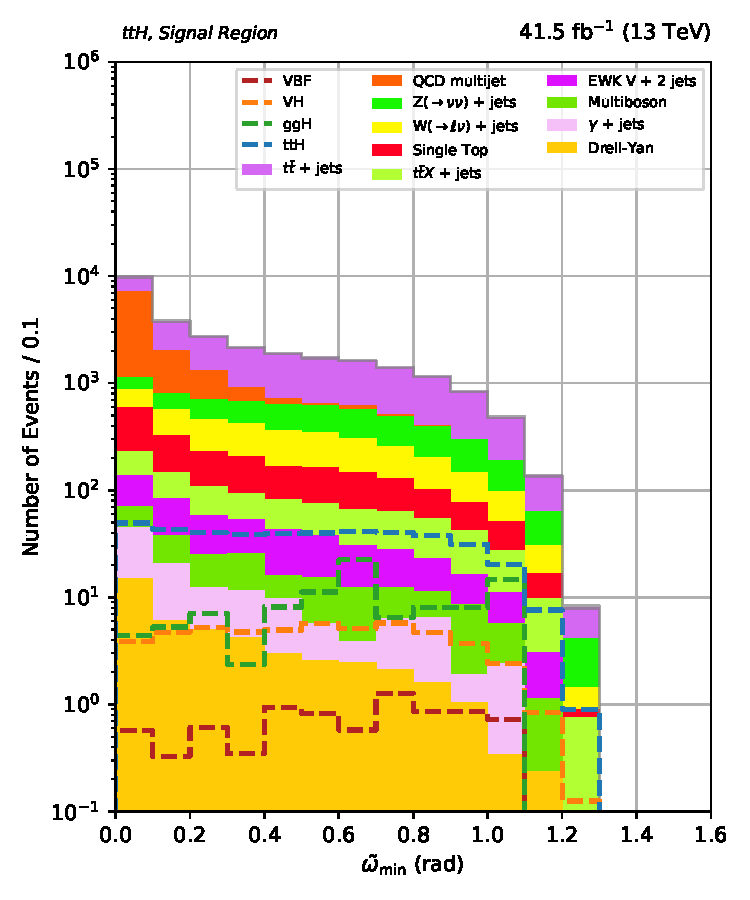
\includegraphics[width=\textwidth]{figures/category_optimisations/with_mindphi_cut/min_omega_tilde_ttH.pdf}
        \caption{\ttH channel}
    \end{subfigure}
    \hspace{0.1\textwidth}
    \begin{subfigure}[b]{0.35\textwidth}
        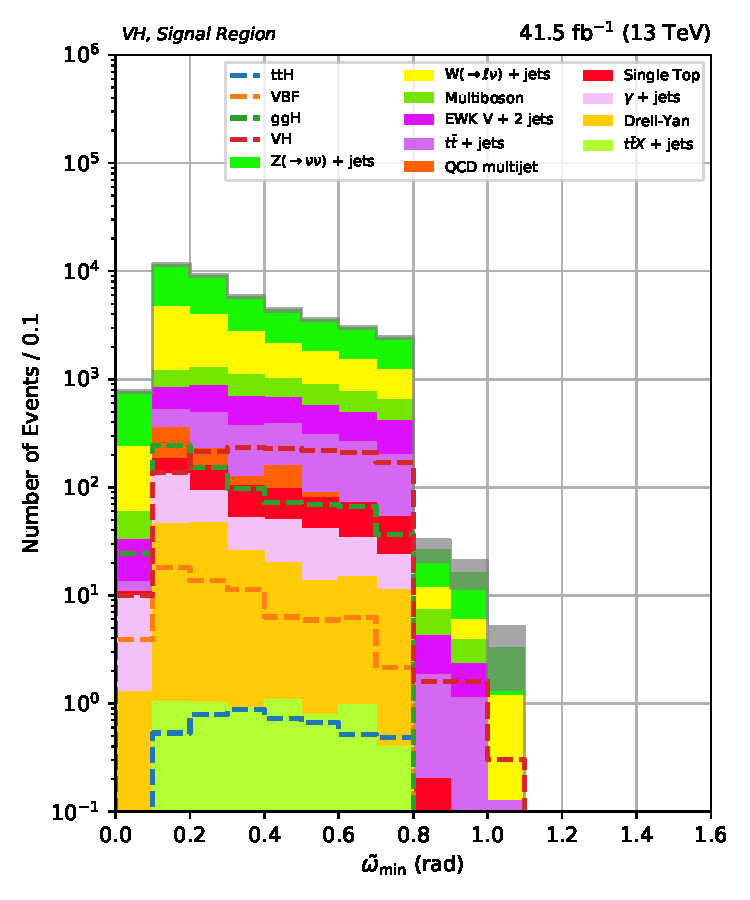
\includegraphics[width=\textwidth]{figures/category_optimisations/with_mindphi_cut/min_omega_tilde_VH.pdf}
        \caption{\VH channel}
    \end{subfigure}

    \begin{subfigure}[b]{0.35\textwidth}
        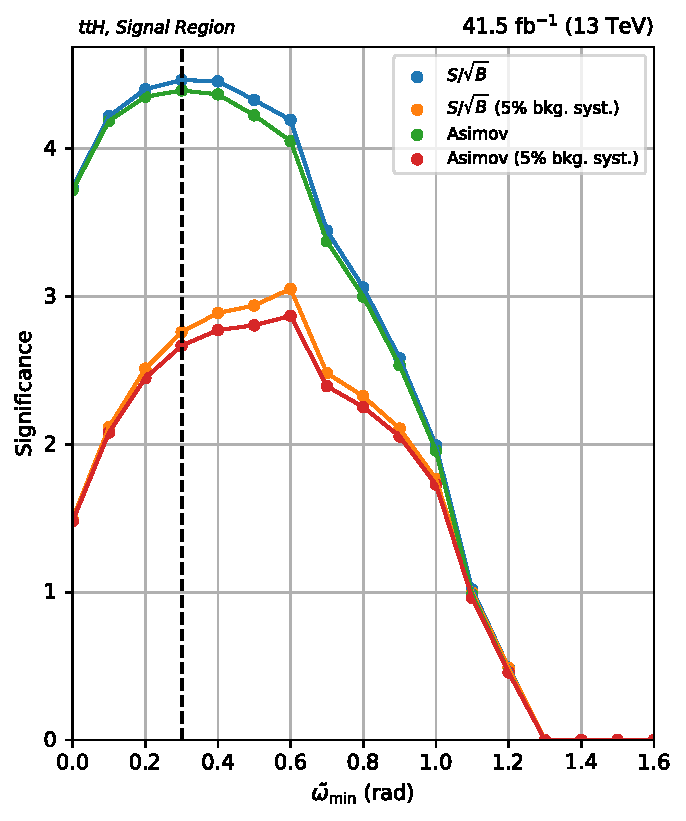
\includegraphics[width=\textwidth]{figures/category_optimisations/with_mindphi_cut/significance_ttH_min_omega_tilde_all.pdf}
        \caption{Significance of cut in \ttH channel}
    \end{subfigure}
    \hspace{0.1\textwidth}
    \begin{subfigure}[b]{0.35\textwidth}
        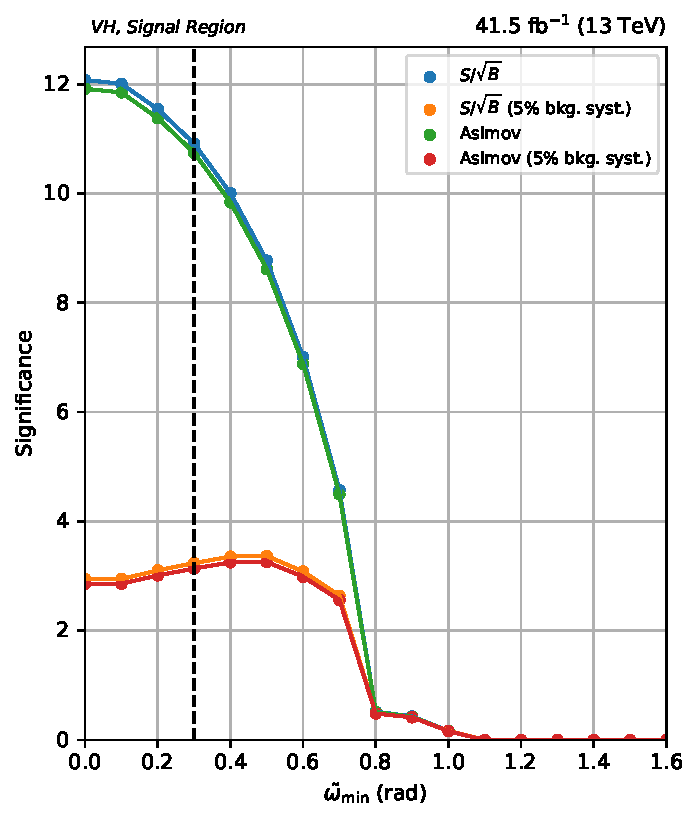
\includegraphics[width=\textwidth]{figures/category_optimisations/with_mindphi_cut/significance_VH_min_omega_tilde_all.pdf}
        \caption{Significance of cut in \VH channel}
    \end{subfigure}
    \caption[Distributions of \omegaTilde in the signal region in the \ttH and \VH categories, along with the significance---from several figures of merit---if a cut is placed to the right of a given value]{Top row: distributions of \omegaTilde in the signal region in the \ttH and \VH categories. Bottom row: the significance---from several figures of merit---if a cut is placed to the right of a given value of \omegaTilde in each production mechanism. The black dotted line indicates the threshold used in the analysis. These are showcased after the analysis-level selection on signal and background simulation for the 2017 data-taking era.}
    \label{fig:htoinv_category_optimisations_significances}
\end{figure}

% Figures from 12th August 2020, scenario 5. When remaking, ensure the colours of the signal lines are consistent, and the legend doesn't overlap with the distribution

It is obvious that the shapes and magnitudes of the significance distributions are sensitive to the inclusion of an estimated systematic uncertainty. Increasing its size affects the shape little, though impacts the magnitude more significantly. In bins with high background occupancy, even a small systematic uncertainty can wash out traces of signal. The thresholds chosen for \omegaTilde do not necessarily maximise the significance---where the Asimov method with $\bkgsystuncert = \text{5\,\%}$ was the leading choice---but to sufficiently separate signal and background, while not removing too many events. The \glspl{CR} in the analysis perform better estimations of their responsible backgrounds when adequately populated. Reducing the event counts in the \glspl{CR} too greatly with the \omegaTilde cut can therefore cause problems in multiple aspects of the analysis.


%=========================================================


\subsubsection{Other optimisations}
\label{subsubsec:htoinv_other_optimisations}

In the ``background rejection'' column of Tab.~\ref{tab:htoinv_categories}, selections were made to distinguish signal from leading backgrounds. The \ttH resolved categories employ requirements on the azimuthal angle between the missing transverse momentum and either the leading jet, leading \Pbottom-jet, or subleading \Pbottom-jet. These are specifically to differentiate \ttH signal from \ttbar background, as the former has been shown to exhibit larger separation between the \glspl{jet} and \ptmiss than the latter. A window on the dijet mass is applied to the \VH resolved categories to reconstruct the \PW and \PZ mass. The 15\GeV below $m_{\PW}$ and above $m_{\PZ}$ allow some leeway to accommodate \glspl{jet} resolution effects. A tight window also acts as an extra multijet background suppressor.


%=========================================================


\subsection{Binning}
\label{subsec:htoinv_binning}

In addition to the categories in Chpt.~\ref{sec:htoinv_categorisation}, events are further separated into bins of \ptmiss as that distribution is expected to maximally differentiate signal and background in the fit. Since the number of events can significantly differ between categories in the different regions of the analysis, the number and widths of the bins are tuned to ensure sufficient statistical precision. These schemes are tied to the category, so are reflected in all regions such that the background estimation methods can operate on a bin-by-bin basis. The binning configuration is outlined in Tab.~\ref{tab:htoinv_binning_scheme}.

\begin{table}[htbp]
    \centering
    \begin{tabular}{ccl}
        \toprule
        Channel & Category & \ptmiss bins (GeV) \\\midrule
        \multirow{9}{*}{\ttH} & 2Boosted & [200, 300), [300, 400), [400, $\infty$) \\
        & 1t1b & [200, 300), [300, 400), [400, $\infty$) \\
        & 1t2b & [200, 300), [300, 400), [400, 600), [600, $\infty$) \\
        & 1W1b & [200, 300), [300, 400), [400, $\infty$) \\
        & 1W2b & [200, 300), [300, 400), [400, $\infty$) \\
        & 5j1b & [200, 300), [300, 400), [400, $\infty$) \\
        & 6j1b & [200, 300), [300, 400), [400, $\infty$) \\
        & 5j2b & [200, 300), [300, 400), [400, $\infty$) \\
        & 6j2b & [200, 300), [300, 400), [400, $\infty$) \\
        \midrule
        \multirow{4}{*}{\VH} & 2j0b & [200, 300), [300, 400), [400, $\infty$) \\
        & 2j1b & [200, 300), [300, 400), [400, $\infty$) \\
        & 2j2b & [200, $\infty$)\\
        & 1V & [200, 300), [300, 400), [400, $\infty$) \\
        \bottomrule
    \end{tabular}
    \caption[The binning scheme implemented to categorise events in terms of \ptmiss]{The binning scheme implemented to categorise events in terms of \ptmiss.}
    \label{tab:htoinv_binning_scheme}
\end{table}


%=========================================================


\subsection{The signal region}
\label{subsec:htoinv_signal_region}

The signal region is the area of phase space where the highest rate of invisible Higgs boson decays are expected to manifest, and the background to be reduced sufficiently that the potential presence of signal in data can be statistically verified. In this analysis, only hadronic final states are permitted. Events with leptons, photons and taus meeting the loose or veto criteria in Chpt.~\ref{sec:analysis_objects} are vetoed.

Events must satisfy a logical \texttt{OR} of \acrshort{hlt} cross-triggers for \acrlong{pf} \ptmiss and \mht calculated without muons (as they can also appear in the \gls{jet} collection in \acrshort{cms}), and at least one \gls{jet} fulfilling the tight ID criteria (see Chpt.~\ref{sec:analysis_objects}). The triggers are illustrated in Tab.~\ref{tab:htoinv_SR_triggers}.

\begin{table}[htbp]
    \centering
    \begin{tabular}{ccccc}
        \toprule
        Year & $\ptmissNoMu$ (\GeVns) & $\mhtNoMu$ (\GeVns) & $\HT$ (\GeVns) & $\njet$ with tight ID \\ \midrule
        \multirow{4}{*}{2016} & 90 & 90 & --- & $\geq \text{1}$ \\
        & 100 & 100 & --- & $\geq \text{1}$ \\
        & 110 & 110 & --- & $\geq \text{1}$ \\
        & 120 & 120 & --- & $\geq \text{1}$ \\
        \midrule
        \multirow{2}{*}{2017} & 120 & 120 & --- & $\geq \text{1}$ \\
        & 120 & 120 & 60 & $\geq \text{1}$ \\
        \midrule
        2018 & 120 & 120 & --- & $\geq \text{1}$ \\
        \bottomrule
    \end{tabular}
    \caption[The trigger thresholds required for events to enter the signal region in each data taking year]{The trigger thresholds required for events to enter the signal region in each data taking year. Each quantity is computed with the \gls{particleflow} at \acrshort{hlt} level. The variables \ptmiss and \mht do not include muons in the calculations.}
    \label{tab:htoinv_SR_triggers}
\end{table}

The relative composition in each category of the signal region (after the event selection) for signal and background are illustrated in Fig.~\ref{fig:htoinv_sr_composition_comb2016to18}, highlighting the effectiveness to which the categories capture the targeted topologies, and the dominant background processes, respectively. The \ttH categories, especially those designed to tag boosted top quarks and vector bosons are very pure in \ttH. Similarly, the \VH categories predominantly consist of events from the production mode of focus. Contamination from the \acrshort{vbf} process is present at a low level, most notably in the resolved categories given the similar topologies. \ggH signal permeates several categories as the second largest component. This is likely due to its high cross section (more than ten times any other individual process) and its ability to mimic the final states of the other signals. \ttbarpjets is the dominant background for the \ttH categories as expected, with \ztonunupjets leading in the others. \wtolnupjets also contributes a reasonable fraction. 

\begin{figure}[htbp]
    \centering
    \begin{subfigure}[b]{0.4\textwidth}
        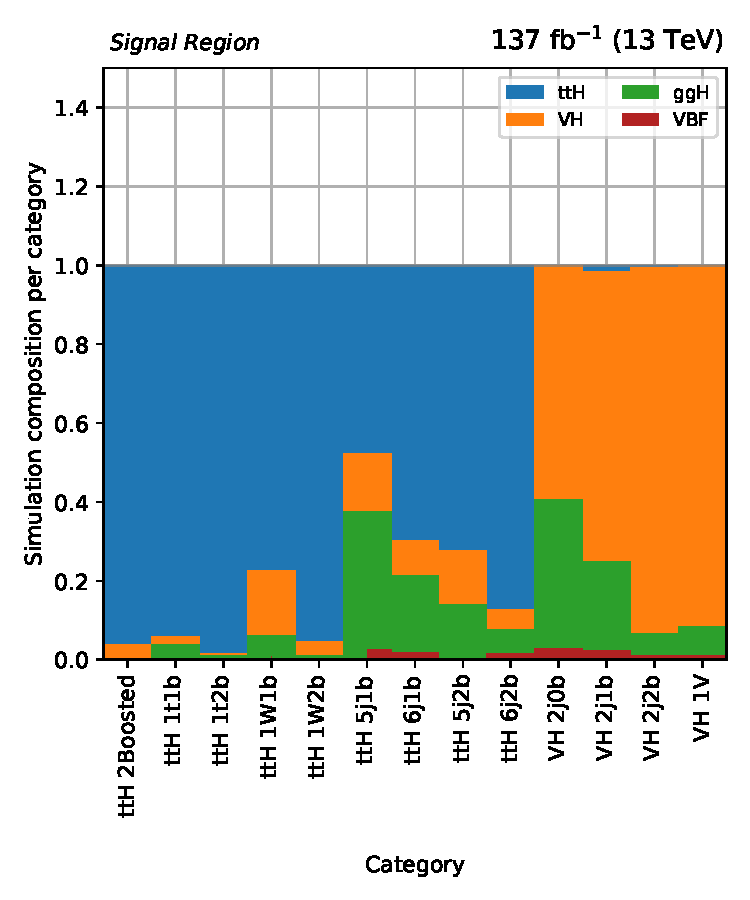
\includegraphics[width=\textwidth]{figures/region_plots/full_Run2/region_0/signal_composition.pdf}
        \caption{Signal composition}
    \end{subfigure}
    \hspace{0.05\textwidth}
    \begin{subfigure}[b]{0.4\textwidth}
        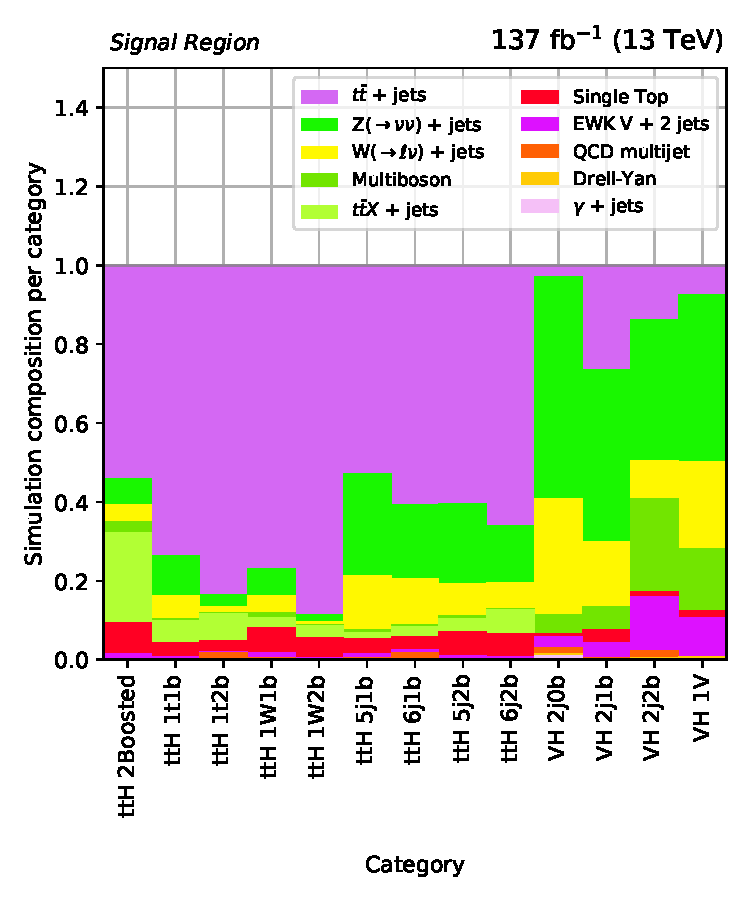
\includegraphics[width=\textwidth]{figures/region_plots/full_Run2/region_0/background_composition.pdf}
        \caption{Background composition}
    \end{subfigure}
    \caption[Composition of each category in the signal region for simulated signal and background processes after the analysis-level selection]{Composition of each category in the signal region for simulated signal and background processes after the analysis-level selection.}
    \label{fig:htoinv_sr_composition_comb2016to18}
\end{figure}
